\section{Funzioni  polinomiali}
\subsection{Fattorizzazione}

\begin{questions}

\question 
\exonly{
	Scomporre in fattori e determinare le soluzioni delle seguenti equazioni:
}
\begin{parts}

\part
\exonly{$x^3-x^2-10x-8=0$}
\solonly{$(x + 1) (x + 2) (x - 4)=0$ \\ $S=\left\lbrace -2,-1,4\right\rbrace $}

\part
\exonly{$x^3 + x^2 -14x -24 = 0$ }
\solonly{$(x - 4) (x + 2) (x + 3) = 0=0$ \\ $S=\left\lbrace -3,-2,4\right\rbrace $}

\part
\exonly{$2 x^3 - 3 x^2 - 17 x + 30 = 0$ }
\solonly{$(x - 2) (x + 3) (2 x - 5) = 0$ \\$S=\left\lbrace -3,2,\dfrac{5}{2}\right\rbrace $}

\part
\exonly{$12x^3+8x^2-3x-2=0$ }
\solonly{ $(3x+2)(2x-1)(2x+1)=0 $ \\ $S=\left\lbrace -\dfrac{2}{3},-\dfrac{1}{2},\dfrac{1}{2}\right\rbrace $ }

\end{parts}	
\begin{profonly}	Src: Swok ex 15-18 impairs pg 289\end{profonly}
	
%	\question
%	\exonly{Favre, ex. 27, pg.219}\sol{Sol. Favre}	
\end{questions}

\subsection{Studio della funzione}

\begin{questions}
\question 
\exonly{
	Realizzare lo studio della funzione (zeri, massimi, minimi, etc.) e rappresentarla graficamente:

}
\begin{parts}

\part
\exonly{$f_1(x)=x^3-x^2-10x-8$}
\ifprintanswers 
%\documentclass[preview,finale]{standalone}
%\usepackage{FulvioCustomIta}

%\begin{document}
\begin{tikzpicture}[baseline={($(current bounding box.north)-(0,1.6ex)$)}]
\tikzset{
	every pin/.style={fill=yellow!50!white,rectangle,rounded corners=3pt,font=\tiny},
	small dot/.style={fill=black,circle,scale=0.3}
}
\begin{axis}[
AxisDefaults, 
width=10cm,
ytick distance={10}]
\addplot[draw=red,smooth,unbounded coords=jump,restrict y to domain=-25:20]{x^3-x^2-10*x-8}; 
\addplot[mark=*] coordinates {(-1.52,1.38)} node[small dot,pin={[pin distance=0.5cm]90:{$(-1.52,1.38)$}}]{} ;
\addplot[mark=*] coordinates {(2.19,-24.2)} node[small dot,pin={[pin distance=1cm]90:{$(2.19,-24.2)$}}]{} ;
\end{axis}
\end{tikzpicture} 
%\end{document}
%\begin{tikzpicture}[baseline={($(current bounding box.north)-(0,1.6ex)$)}]
%  \tikzset{
%	every pin/.style={fill=yellow!50!white,rectangle,rounded corners=3pt,font=\tiny},
%	small dot/.style={fill=black,circle,scale=0.3}
%}
%\begin{axis}[
%AxisDefaults, 
%width=10cm,
%ytick distance={10}]
%\addplot[draw=red,smooth,unbounded coords=jump,restrict y to domain=-25:20]{x^3-x^2-10*x-8}; 
%\addplot[mark=*] coordinates {(-1.52,1.38)} node[small dot,pin={[pin distance=0.5cm]90:{$(-1.52,1.38)$}}]{} ;
%\addplot[mark=*] coordinates {(2.19,-24.2)} node[small dot,pin={[pin distance=1cm]90:{$(2.19,-24.2)$}}]{} ;
%\end{axis}
%\end{tikzpicture} 
\fi


\part
\exonly{$f_2(x)=-x^3 - x^2 +14x +24$ }
\ifprintanswers 
\documentclass[preview,finale]{standalone}
\usepackage{FulvioCustomIta}

\begin{document}
\begin{tikzpicture}[baseline={($(current bounding box.north)-(0,1.6ex)$)}]
\tikzset{
	every pin/.style={fill=yellow!50!white,rectangle,rounded corners=3pt,font=\tiny},
	small dot/.style={fill=black,circle,scale=0.3}
}
\begin{axis}[
AxisDefaults, 
width=10cm,
ytick distance={10}]
\addplot[draw=red,smooth,unbounded coords=jump,restrict y to domain=-45:5]{x^3+x^2-14*x-24}; 
\addplot[mark=*] coordinates {(-2.5,1.6)} node[small dot,pin={[pin distance=2cm]-90:{$(-2.5,1.6)$}}]{} ;
\addplot[mark=*] coordinates {(1.85,-40.1)} node[small dot,pin={[pin distance=1cm]90:{$(1.85,-40.1)$}}]{} ;
\end{axis}
\end{tikzpicture} 
\end{document}
%\begin{tikzpicture}[baseline={($(current bounding box.north)-(0,1.6ex)$)}]
%\tikzset{
%	every pin/.style={fill=yellow!50!white,rectangle,rounded corners=3pt,font=\tiny},
%	small dot/.style={fill=black,circle,scale=0.3}
%}
%\begin{axis}[
%AxisDefaults, 
%width=10cm,
%ytick distance={10}]
%\addplot[draw=red,smooth,unbounded coords=jump,restrict y to domain=-45:5]{x^3+x^2-14*x-24}; 
%\addplot[mark=*] coordinates {(-2.5,1.6)} node[small dot,pin={[pin distance=2cm]-90:{$(-2.5,1.6)$}}]{} ;
%\addplot[mark=*] coordinates {(1.85,-40.1)} node[small dot,pin={[pin distance=1cm]90:{$(1.85,-40.1)$}}]{} ;
%\end{axis}
%\end{tikzpicture} 
\fi


\part
\exonly{$f_3(x)=2 x^3 - 3 x^2 - 17 x + 30 $ }
\ifprintanswers 
%\documentclass[preview,finale]{standalone}
%\usepackage{FulvioCustomIta}

%\begin{document}
\begin{tikzpicture}[baseline={($(current bounding box.north)-(0,1.6ex)$)}]
\tikzset{
	every pin/.style={fill=yellow!50!white,rectangle,rounded corners=3pt,font=\tiny},
	small dot/.style={fill=black,circle,scale=0.3}
}
\begin{axis}[
AxisDefaults, 
width=10cm,
ytick distance={10}]
\addplot[draw=red,smooth,unbounded coords=jump,restrict y to domain=-5:45]{2*x^3-3*x^2-17*x+30}; 
\addplot[mark=*] coordinates {(-1.26,42.66)} node[small dot,pin={[pin distance=2cm]-90:{$(-1.26,42.66)$}}]{} ;
\addplot[mark=*] coordinates {(2.26,-0.66)} node[small dot,pin={[pin distance=1cm]90:{$(2.26,-0.66)$}}]{} ;
\end{axis}
\end{tikzpicture} 
%\end{document}
%\begin{tikzpicture}[baseline={($(current bounding box.north)-(0,1.6ex)$)}]
%\tikzset{
%	every pin/.style={fill=yellow!50!white,rectangle,rounded corners=3pt,font=\tiny},
%	small dot/.style={fill=black,circle,scale=0.3}
%}
%\begin{axis}[
%AxisDefaults, 
%width=10cm,
%ytick distance={10}]
%\addplot[draw=red,smooth,unbounded coords=jump,restrict y to domain=-5:45]{2*x^3-3*x^2-17*x+30}; 
%\addplot[mark=*] coordinates {(-1.26,42.66)} node[small dot,pin={[pin distance=2cm]-90:{$(-1.26,42.66)$}}]{} ;
%\addplot[mark=*] coordinates {(2.26,-0.66)} node[small dot,pin={[pin distance=1cm]90:{$(2.26,-0.66)$}}]{} ;
%\end{axis}
%\end{tikzpicture} 
\fi



\part
\exonly{$f_4(x)=12x^3+8x^2-3x-2$ }
\ifprintanswers 
\begin{tikzpicture}[baseline={($(current bounding box.north)-(0,1.6ex)$)}]
\tikzset{
	every pin/.style={fill=yellow!50!white,rectangle,rounded corners=3pt,font=\tiny},
	small dot/.style={fill=black,circle,scale=0.3}
}
\begin{axis}[
AxisDefaults, 
width=10cm,
ytick distance={1}]
\addplot[draw=red,smooth,unbounded coords=jump,restrict y to domain=-10:10]{12*x^3+8*x^2-3*x-2}; 
\addplot[mark=*] coordinates {(-0.59,0.09)} node[small dot,pin={[pin distance=2cm]-90:{$(-0.59,0.09)$}}]{} ;
\addplot[mark=*] coordinates {(0.14,-2.23)} node[small dot,pin={[pin distance=1cm]90:{$(0.14,-2.23)$}}]{} ;
\end{axis}
\end{tikzpicture} 
\fi









	
\end{parts}	

\solnewpage	
\question	
\exonly{
	Realizzare lo studio delle funzioni seguenti (zeri e molteplicità, rappresentazione grafica).}

\begin{parts}
\part
\exonly{$f(x)=x^4-4x^2$}
\solonly{Zero: $0$ molteplicità $2$, $2$ molt. $1$ et $-2$ molt. $1$}

	\ifprintanswers 
	\begin{tikzpicture}[baseline={($(current bounding box.north)-(0,1.6ex)$)}]
	\begin{axis}[AxisDefaults,
	width=12cm,
	ytick distance={1},]
		\addplot[draw=red,smooth,unbounded coords=jump,restrict y to domain=-10:10]{x^4-4*x^2}; 
	\end{axis}
	\end{tikzpicture} 
	\fi
	
	\begin{profonly}	Src: Swok ex 15 pg 260\end{profonly}
	
	\part
	\exonly{$f(x)=-x^3+3x^2+10x$}
	\solonly{Zero: $0$ molteplicità $1$, $5$ molt. $1$ et $-2$ molt. $1$}
	
	\ifprintanswers
		\begin{tikzpicture}[baseline={($(current bounding box.north)-(0,1.6ex)$)}]
		\begin{axis}[AxisDefaults,
		width=12cm,
			ytick distance={10},
			]
			\addplot[draw=red,smooth,unbounded coords=jump,
			restrict y to domain=-20:35,
			domain=-3:6
			]{-x^3+3*x^2+10*x}; 
		\end{axis}
		\end{tikzpicture} 
		\fi
		
		\begin{profonly}	Src: Swok ex 17 pg 260\end{profonly}
	\solnewpage	
\part
	\exonly{$f(x)=\dfrac{1}{6}(x+2)(x-3)(x-4)$}
	\solonly{Zero: $-2$ molteplicità $1$, $3$ molt. $1$ et $4$ molt. $1$}

\ifprintanswers 
	\begin{tikzpicture}[baseline={($(current bounding box.north)-(0,1.6ex)$)}]
	\begin{axis}[AxisDefaults,
	width=12cm,
		ytick distance={1},
		]
		\addplot[draw=red,smooth,unbounded coords=jump,
		restrict y to domain=-5:5,
		domain=-3:6
		]{(x+2)*(x-3)*(x-4)/6}; 
	\end{axis}
	\end{tikzpicture} 
\fi
	
	\begin{profonly}	Src: Swok ex 19 pg 260\end{profonly}	
	
\part
	\exonly{$f(x)=-x^3-2x^2+4x+8$}
	\solonly{Zero: $2$ molteplicità $1$, $-2$ molt. $2$}
	
	\ifprintanswers 	
	\begin{tikzpicture}[baseline={($(current bounding box.north)-(0,1.6ex)$)}]
		\begin{axis}[AxisDefaults,
		width=12cm,
			ytick distance={2},
			]
			\addplot[draw=red,smooth,unbounded coords=jump,
			restrict y to domain=-10:10,
			domain=-3:6
			]{-x^3-2*x^2+4*x+8}; 
		\end{axis}
		\end{tikzpicture} 
		\fi
		
	\begin{profonly}	Src: Swok ex 21 pg 260\end{profonly}
		
		
						
					
\solnewpage
\part
	\exonly{$f(x)=x^4-6x^2+8$}
	\solonly{Zero: $2$ molteplicità $1$, $-2$ molt. $1$, $\sqrt{2}$ molt. $1$ e $-\sqrt{2}$ molt. $1$.}
	
		\ifprintanswers 
		\begin{tikzpicture}[baseline={($(current bounding box.north)-(0,1.6ex)$)}]
		\begin{axis}[AxisDefaults,
		width=12cm,
			ytick distance={2},
			ymin=-3,
			]
			\addplot[draw=red,smooth,unbounded coords=jump,
			restrict y to domain=-10:10,
			%domain=-3:6
			]{x^4-6*x^2+8}; 
		\end{axis}
		\end{tikzpicture} 
		\fi
		
	\begin{profonly}	Src: Swok ex 23 pg 260\end{profonly}


\part
	\exonly{$f(x)=x^2(x+1)^2(x-2)(x-4)$}
	\solonly{Zero: $0$ molteplicità $2$, $-1$ molt. $2$, $2$ molt. $1$ e $4$ molt. $1$.}
	
		\ifprintanswers 
		\begin{tikzpicture}[baseline={($(current bounding box.north)-(0,1.6ex)$)}]
		\begin{axis}[AxisDefaults,
			width=12cm,
			ytick distance={5},
			ymin=-10,
			ymax=20,
			xmax=5,
			]
			\addplot[draw=red,smooth,
			restrict y to domain=-20:40,
			domain=-5:3.2,
			]{x^2*(x+1)^2*(x-2)*(x-4)}; 
			\addplot[draw=red,smooth,
			restrict y to domain=-20:40,
			domain=3.5:5,
			]{x^2*(x+1)^2*(x-2)*(x-4)}; 
		\end{axis}
		\end{tikzpicture} 
		\fi
		
	\begin{profonly}	Src: Swok ex 25 pg 260\end{profonly}	
		
		
		\solnewpage			
\part
	\exonly{$f(x)=12x^3-4x^2-3x+1$}
	\solonly{Zero: $\frac{1}{3}$ molteplicità $1$, $\frac{1}{2}$ molt. $1$ e $-\frac{1}{2}$ molt. $1$}
	
	\ifprintanswers 
		\begin{tikzpicture}[baseline={($(current bounding box.north)-(0,1.6ex)$)}]
		\begin{axis}[AxisDefaults,
			width=12cm,
			ytick distance={0.5},ytick distance={0.5},
			xmin=-1.2,xmax=1.2,
			ymin=-0.5,ymax=1.5,
			]
			\addplot[draw=red,smooth,unbounded coords=jump,
			restrict y to domain=-10:10,
			domain=-3:6
			]{12*x^3-4*x^2-3*x+1}; 
		\end{axis}
		\end{tikzpicture} 
		\fi	
\end{parts}
	
\end{questions}

\exnewpage
\subsection{Rappresentazione grafica}

\begin{questions}

\question 
	\exonly{
		Determinare la funzione polinomiale di 3° grado rappresentata qui sotto.}
	\solonly{$f(x)=\dfrac{7}{9}(x+1)(x-\dfrac{3}{2})(x-3)$}

	\begin{tikzpicture}[baseline={($(current bounding box.north)-(0,1.6ex)$)}]
		\exonly{
	\begin{axis}[AxisDefaults,
	width=0.7\linewidth,
	xlabel=$t$, xlabel style={at=(current axis.right of origin), anchor=west},
		ylabel=$N(t)$, ylabel style={at=(current axis.above origin), anchor=south},
		ytick distance={1},
		grid=both,
		minor tick num = 1,
		ymin=-5,ymax=5,xmin=-2,xmax=5,
		]
		\addplot[draw=red,thick,smooth,unbounded coords=jump,
		restrict y to domain=-7:6,
		domain=-5:5
		]{7*(x+1)*(x-3/2)*(x-3)/9}; 
		%\filldraw (axis cs:0,3.5) circle (1.5pt) node[above right] {\tiny $(0;\num{3.5})$};
	\end{axis}
	
	}
	\end{tikzpicture}
					
					

\begin{profonly}	Src: Swok ex 11 pg 280\end{profonly}

\question 
\exonly{
	Determinare la funzione polinomiale di 4° rappresentata qui sotto.}
\solonly{$f(x)=\dfrac{1}{12}x(x-1)(x-3)(x-5)$}

\begin{tikzpicture}[baseline={($(current bounding box.north)-(0,1.6ex)$)}]
	\exonly{
\begin{axis}[AxisDefaults,
width=0.7\linewidth,
	ytick distance={1},
	grid=both,
	minor tick num = 1,
	ymin=-2,ymax=6,xmin=-3,xmax=6,
	]
	\addplot[draw=red,thick,smooth,unbounded coords=jump,
	restrict y to domain=-3:8,
	domain=-3:7
	]{x*(x-1)*(x-3)*(x-5)/12}; 
	\addplot [only marks, mark=o] (1,-4) node[left] {\scriptsize $(-1;\num{4})$} ;
	%\filldraw (axis cs:-1,4) circle (1.5pt) node[left] {\scriptsize $(-1;\num{4})$};
\end{axis}

}
\end{tikzpicture}
					
	

\begin{profonly}	Src: Swok ex 12 pg 280\end{profonly}
\exnewpage

\question 
\exonly{
	Determinare la funzione polinomiale rappresentata qui sotto. In seguito determinare massimi e minimi locali alla calcolatrice.}


\begin{parts}
\part

	\solonly{$f(x)=-(x-1)^2(x-3)$ 
	\newline
	Massimo locale $(2.33;119)$ , Minimo locale $(1;0)$

	}
	
\begin{tikzpicture}[baseline={($(current bounding box.north)-(0,1.6ex)$)}]
\exonly{
\begin{axis}[AxisDefaults,
width=0.7\linewidth,
ytick distance={1},
grid=both,
minor tick num = 1,
ymin=-2,ymax=6,xmin=-3,xmax=6,
]
\addplot[draw=red,thick,smooth,unbounded coords=jump,
restrict y to domain=-3:8,
domain=-3:7
]{-(x-3)*(x-1)^2}; 

\end{axis}

}
\end{tikzpicture}



\begin{profonly}	Src: Swok ex 13 pg 280\end{profonly}

%\question 
%\exonly{Déterminer la fonctions polynomiale dont le graphique est donne sur la figure}
\part
\solonly{$f(x)=(x-2)^2(x-4)$
	\newline
Massimo locale $(2;0)$ , Minimo locale $(3.33;-1.19)$
}

\begin{tikzpicture}[baseline={($(current bounding box.north)-(0,1.6ex)$)}]
\exonly{
\begin{axis}[AxisDefaults,
width=0.7\linewidth,
ytick distance={1},
grid=both,
minor tick num = 1,
ymin=-5,ymax=5,xmin=-2,xmax=6,
]
\addplot[draw=red,thick,smooth,unbounded coords=jump,
restrict y to domain=-6:6,
domain=-3:7
]{(x-4)*(x-2)^2}; 
	\addplot [only marks, mark=o] (1,-3) node[right] {\scriptsize $(-1;3)$} ;
%\filldraw (axis cs:1,-3) circle (1.5pt) node[right] {\scriptsize $(1;-3)$};
\end{axis}

}
\end{tikzpicture}

\part
\solonly{$f(x)=\dfrac{1}{512}(x-2)^2(x+2)^2(x-8)^2$
\newline Massimi locali $(-0.24;2.06)$, $(5.57;8.42)$ \newline
Minimi globali $(-2;0)$, $(2;0)$ e $(8;0)$
}

\begin{tikzpicture}[baseline={($(current bounding box.north)-(0,1.6ex)$)}]
\exonly{
	\begin{axis}[AxisDefaults,
	width=0.7\linewidth,
	ytick distance={1},
	grid=both,
	minor tick num = 1,
	ymin=-2,ymax=11,xmin=-4,xmax=10,
	]
	\addplot[draw=red,thick,smooth,unbounded coords=jump,
	restrict y to domain=-2:15,
	domain=-4:11
	]{1/512*(x-2)^2*(x+2)^2*(x-8)^2}; 
		\addplot [only marks, mark=o] (0,2) node[right] {\scriptsize $(0;2)$};
	%\filldraw (axis cs:0,2) circle (1.5pt) node[right] {\scriptsize $(0;2)$};
	\end{axis}
	
}
\end{tikzpicture}

\begin{profonly}	Src: Swok ex 14 pg 280\end{profonly}
\end{parts}


%\question
%\exonly{Favre, ex. 24, pg.218}	
%\solonly{Sol. Favre}
\solnewpage


	\question
	 \exonly{Risolvere la seguente equazione utilizzando un metodo grafico: $x^3 = 0.6x + 3$ . 
	 Si cerchi dapprima una 	soluzione approssimata determinando l’intersezione tra i grafici di $f (x) = x^3$  e $g(x) = 0.6x + 3$. 
	 
	 In seguito si confronti il risultato con la soluzione numerica data dalla calcolatrice.}
	 %TODO: controllare immagine che da errore in compilazione su OSX !!!!!
 \solonly{
	 \begin{tikzpicture}[baseline={($(current bounding box.north)-(0,1.6ex)$)}]
	 \begin{axis}[AxisDefaults,
	 width=0.7\linewidth,
	 ytick distance={1},
	 grid=both,
	 minor tick num = 1,
	 ymin=-3,ymax=5,xmin=-2,xmax=3,
	 domain=-3:3
	 ]
	 \addplot[draw=blue,thick,smooth,unbounded coords=jump,
	 restrict y to domain=-6:6,name path=cubic ]{(x^3}; 
	\addplot[draw=red,thick,smooth,unbounded coords=jump,
	 restrict y to domain=-6:6,name path=line 
	 ]{0.6*x+3}; 
	 	 \path [name intersections={of=cubic and line, by=a}];
	 	\path (a) node[pin={[pin distance=1cm]-80:{$\approx(1.6;4)$}}]{} ;
	 \end{axis}

	 \end{tikzpicture}
	Calcolatrice: $\es{(\num{1.5805},4)}$
	}

\exnewpage
\question
\exonly{Dato il grafico di $f(x)$ risolvere graficamente l'equazione $f(x)=3$.

%Last revision: 14.09.2020
%CHANGELOG: assi più visibili, very thick e black
% major grid più visibile black!50 e thick


\begin{tikzpicture}[baseline={($(current bounding box.north)-(0,1.6ex)$)}]
\begin{axis}[AxisDefaults,
major grid style={ thick,black!50},
axis line style={very thick, black},
x=1.5cm,y=1.5cm,
%width=\linewidth,
ytick distance={1},
grid=both,
minor tick num = 9,
ymin=-5,ymax=7,xmin=-4,xmax=5,
domain=-4:5
]
\addplot[draw=blue,thick,smooth,unbounded coords=jump,
restrict y to domain=-6:8]{(x+3)*(x+1)*(x-2)*(x-1)*(x-4)/12.5}; 
\end{axis}
\end{tikzpicture}
}

\exnewpage
\question
\exonly{Dato il grafico di $f(x)$ risolvere graficamente l'equazione $ f(x) + \frac{3}{4}x=3$.
	
	%Last revision: 14.09.2020
%CHANGELOG: assi più visibili, very thick e black
% major grid più visibile black!50 e thick


\begin{tikzpicture}[baseline={($(current bounding box.north)-(0,1.6ex)$)}]
\begin{axis}[AxisDefaults,
major grid style={ thick,black!50},
axis line style={very thick, black},
x=1.5cm,y=1.5cm,
%width=\linewidth,
ytick distance={1},
grid=both,
minor tick num = 9,
ymin=-5,ymax=7,xmin=-4,xmax=5,
domain=-4:5
]
\addplot[draw=blue,thick,smooth,unbounded coords=jump,
restrict y to domain=-6:8]{(x+3)*(x+1)*(x-2)*(x-1)*(x-4)/12.5}; 
\end{axis}
\end{tikzpicture}
}
\exnewpage


	
	
	
	\question
	Per ogni grafico sono proposte quattro funzioni da $\R \longrightarrow \R$. Associare la legge di assegnazione con il grafico.
	
	
	\begin{parts}
		\part
		\begin{tikzpicture}[baseline={($(current bounding box.north)-(0,1.6ex)$)}]
		\begin{axis}[AxisDefaults,
		width=8cm,
		ymin=-3,ymax=3,xmin=-1,xmax=3,
		grid=none,
		xtick = \empty,
		ytick = \empty,
		]
		\addplot[draw=red,smooth,unbounded coords=jump,
		restrict y to domain=-6:6,
		domain=-1:5
		]{3*x*(x-1)*(x-2)}; 
		\end{axis}
		\end{tikzpicture} 
		\begin{minipage}[t][][c]{0.5\linewidth}
			$f_1(x)=x^2(x-1)^2(x-2)$  \medskip 
			
			$f_2(x)=3x(x-1)(x-2)$ \medskip
			
			$f_3(x)=x^3(x-1)(x-2)$\medskip
			
			$f_4(x)=-x(x-1)(x-2)$
		\end{minipage}
		
		\part
		\begin{tikzpicture}[baseline={($(current bounding box.north)-(0,1.6ex)$)}]
		\begin{axis}[AxisDefaults,
		width=8cm,
		ymin=-3,ymax=3,xmin=-1,xmax=3,
		grid=none,
		xtick = \empty,
		ytick = \empty,
		]
		\addplot[draw=red,smooth,unbounded coords=jump,
		restrict y to domain=-6:6,
		domain=-1:5
		]{5*x*(x-1)^2*(x-2)}; 
		\end{axis}
		\end{tikzpicture} 
		\begin{minipage}[t][][c]{0.5\linewidth}
			$f_1(x)=2x^3(x-1)(x-2)^2$  \medskip 
			
			$f_2(x)=x^2(x-1)(x-2)$ \medskip
			
			$f_3(x)=5x(x-1)^2(x-2)$\medskip
			
			$f_4(x)=-2x(x-1)(2-x)$
		\end{minipage}
		
		
	\end{parts}

\end{questions}
\exnewpage
\subsection{Applicazioni varie}

\begin{questions}

	\question
	\exonly{Determinare gli zeri nonché il massimo e il minimo locale della seguente funzione:
	
	$f(x)=\num{0.046}x^3-\num{1.57}x^2 +\num{14.3}x-26$
	

	}

	
	


	\solonly{
	Zeri:  $x_1=\num{2.411570}$, $x_2=\num{11.718864}$ e $x_3=\num{20}$ \\
	Massimo locale: $P_{\text{max}}=(\num{6.2966};\num{13.27887}) $\\
	Minimo locale: $P_{\text{min}}=(\num{16.4570};\num{-10.846}) $\\
	}
	
\question 
\exonly{
	Un branco di 100 cervi viene introdotto su di una piccola isola.
%	Un troupeau de 100 cerfs est introduit sur une petite île. 
Inizialmente il branco cresce rapidamente, ma in seguito le risorse cominciano a scarseggiare e la popolazione diminuisce.
%Tout d'abord le troupeau grandit rapidement, mais par la suite les ressources en nourriture baissent et la population diminue.
Supponiamo che il numero di cervi $N(t)$ dopo $t$ anni dalla loro introduzione sull'isola sia dato da  

$N(t) =-t^4 + 21t^2 + 100$, dove $t > 0$.}

\begin{parts}
\part
\exonly{
	Determinare il valore $t$ per il quale $N(t) > 0$ e rappresentare graficamente $N(t)$.
	%Déterminer la valeur de $t$ pour laquelle $N(t) > 0$ et représenter le graphique de $N(t)$.
}
\solonly{$0<t<5$}

\ifprintanswers
 \begin{tikzpicture}[baseline={($(current bounding box.north)-(0,1.6ex)$)}]
\begin{axis}[AxisDefaults,
width=\linewidth,
ytick distance={50},
ymin=0,
]
\addplot[draw=red,smooth,unbounded coords=jump,
restrict y to domain=0:250,
domain=0:5
]{-x^4+21*x^2+100}; 
\end{axis}
\end{tikzpicture} 
\fi
\part
\exonly{
	Secondo questo modello la popolazione si estinguerà? Se si, quando?
%	La population de cerfs va-t-elle s’éteindre? Si oui, quand ?
}
\solonly{
	Si, dopo 5 anni.
}
					
\end{parts}




\question

\exonly{La tabella qui sotto indica la temperatura $\theta$ in \si{\celsius}

misurate nell'arco di una giornata (24 ore).
L'andamento della temperatura in questo intervallo può essere descritto da una funzione polinomiale (di $4\degree$) $f(t)=\theta$.

\begin{tabular}{|c|c|c|c|c|c|}
	\hline 
	$t[\si{\hour}]$  & 0 & 5 & 12 & 19 & 24 \\ 
	\hline 
	$\theta [\si{\celsius}]$ & 0 & 0 & 10 & 0 & 0 \\ 
	\hline 
\end{tabular}  } 

 

\begin{parts}
	\part
	\exonly{Determinare la legge di assegnazione di $f(t)$ e tracciarne l'andamento. }
	\solonly{ $f(t)=\dfrac{5}{3528}t(t-5)(t-19)(t-24)$ }
	
	\part
	\exonly{Determinare la temperatura $\theta $ se $t=9$ }
	\solonly{$ \theta \approx 7.65 \si{\celsius}$ }
\end{parts}


\question
\exonly{La relazione tra la quantità $q$ e il prezzo $p$ ci permettono di descrivere l'offerta e la domanda di un certo bene sul mercato. 

Vorremmo calcolare il prezzo di equilibrio  tra le funzioni di domanda e offerta seguenti:

Offerta: $q=\sqrt{100-\dfrac{300}{p^2}}$

Domanda: $q=\dfrac{2400}{p^2}$
}
\solonly{$p\approx 15.64$ }

\question
\exonly{Determinare il polinomio di Newton $$P_k(x)=c_0+c_1(x-x_0)+\ldots +c_k(x-x_0)\ldots(x-x_{k-1})$$ passante per i punti  $$(1;3) \quad (2;5) \quad (3;1) \quad (6;-3)$$ }
\solonly{$P(x)=3+2(x-1)-3(x-1)(x-2)+\dfrac{11}{15}(x-1)(x-2)(x-3)$ }


%\subfile{../ch/BS-MPT-FP-fct-polyn}


\question

\exonly{
Il cubo grande ha un lato di \SI{10}{\centi\metre}. Si vuole costruire un parallelepipedo a base quadrata come in figura: 


%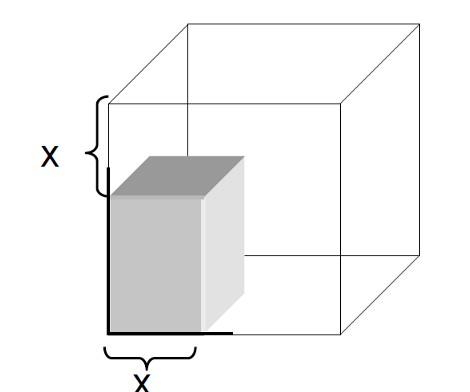
\includegraphics[scale=1]{cubo}

\begin{tikzpicture}[baseline={($(current bounding box.north)-(0,1.6ex)$)}]
%\tikzstyle{isometric}=[x={(0.710cm,-0.410cm)},y={(0cm,0.820cm)},z={(-0.710cm,-0.410cm)}]
%\tikzset{every path/.style={isometric}}
\tikzset{face/.style={fill=gray!20}}
\pgfmathsetmacro{\cubex}{3}
\pgfmathsetmacro{\cubey}{3}
\pgfmathsetmacro{\cubez}{3}
\pgfmathsetmacro{\ratio}{0.4}

\coordinate (FTR) at (0,0,0);
\coordinate (FTL) at (-\cubex,0,0);
\coordinate (FBL) at (-\cubex,-\cubey,0);
\coordinate (FBR) at (0,-\cubey,0);
\coordinate (BTR) at (0,0,-\cubez);
\coordinate (BBR) at (0,-\cubey,-\cubez);
\coordinate (BTL) at (-\cubex,0,-\cubez);
\coordinate (BBL) at (-\cubex,-\cubey,-\cubez);


\draw[dotted] (FTR)  -- (FTL)  -- (FBL)  -- (FBR)  -- cycle;
\draw[dotted] (FTR) -- (BTR)  -- (BTL)  -- (FTL) -- cycle;
\draw[dotted] (FTR) -- (FBR) -- (BBR)  -- (BTR) -- cycle;
\dimline[line style = {line width=0.7},extension start length=-0.5cm,extension end length=-0.5cm] {($(FTL)+(-0.5,0,0)$)}{($(FBL)+(-0.5,0,0)$)}{\SI{10}{\centi\metre}};


\pgfmathsetmacro{\cubex}{1}
\pgfmathsetmacro{\cubey}{2}
\pgfmathsetmacro{\cubez}{1}
%\path (FBR) -- node[midway,right] {$x$}+(0,\cubex,0);
\dimline[line style = {line width=0.7},
extension start length=-0.24,
extension end length=-0.24] {(FBR)}{($ (FBR) + (0,\cubex,0) $)}{$x$};

\coordinate (FTR) at (0,0,0);
\coordinate (FTL) at (-\cubex,0,0);
\coordinate (FBL) at (-\cubex,-\cubey,0);
\coordinate (FBR) at (0,-\cubey,0);
\coordinate (BTR) at (0,0,-\cubez);
\coordinate (BBR) at (0,-\cubey,-\cubez);
\coordinate (BTL) at (-\cubex,0,-\cubez);
\coordinate (BBL) at (-\cubex,-\cubey,-\cubez);


\draw[thick] (FTR)  --(FTL)  -- (FBL)  -- (FBR)  -- cycle;
\draw[thick] (FTR) -- (BTR)  -- (BTL)  -- (FTL) -- cycle;
\draw[thick,face] (FTR) -- (FBR) -- (BBR)  -- (BTR) -- cycle;
\dimline[line style = {line width=0.7},
extension start length=-0.24,
extension end length=-0.24] {(FTR)}{(FTL)}{$x$};


\end{tikzpicture}

Determinare i valori approssimati di $x$ tali per cui il volume del parallelepipedo sia di \SI{147}{\cubic\centi\metre}.
 
SFIDA : Determinare i valori esatti di $x$ tali per cui il volume del parallelepipedo sia di \SI{147}{\cubic\centi\metre}.
 }

\solonly{$7$ e $\dfrac{3+\sqrt{93}}{2}\approx 6.32$ }

\question
\exonly{In una giornata di fine estate la temperatura di \SI{20}{\degreeCelsius}  è stata misurata alle 00h00, alle 09h00 e di nuovo alle 24h00.
	
	La temperatura minima è stata riscontrata alle 04h00 ed era di \SI{17}{\degreeCelsius}.
	
	Stabilire un modello polinomiale, $T(x)$ della temperatura in funzione dell'ora per la suddetta giornata e rappresentarla graficamente. }
\solonly{$T(x)=-\dfrac{3}{400}x(x-9)(x-24)+20$

 \begin{tikzpicture}[baseline={($(current bounding box.north)-(0,1.6ex)$)}]
\begin{axis}[AxisDefaults,
width=\linewidth,
ytick distance={1},
ymin=0,
ymax=30,
ylabel=$T(x)$
]
\addplot[ultra thick,draw=red,smooth,unbounded coords=jump,
restrict y to domain=0:35,
domain=0:24
]{-x*(x-9)*(x-24)*3/400+20}; 
\end{axis}
\end{tikzpicture} 
 }
\end{questions}